\documentclass{article}
\usepackage{amsmath}
\usepackage{amssymb}
\usepackage{amsfonts}
\usepackage{dsfont}
\usepackage{graphicx} % Required for inserting images
\usepackage{listings}
	\lstset{language=R,
    basicstyle=\small\ttfamily,
    stringstyle=\color{green},
    otherkeywords={0,1,2,3,4,5,6,7,8,9},
    morekeywords={TRUE,FALSE},
    deletekeywords={data,frame,length,as,character},
    keywordstyle=\color{blue},
    commentstyle=\color{green},
}
\usepackage{xcolor}
\usepackage{array}
\usepackage[vmargin=2cm,hmargin=2cm]{geometry}


\title{TP1-ADM}
\author{Guillaume Bernard-Reymond et Lorenzo Gaggini}
\date{October 2023}

\begin{document}
\newcommand{\norme}[1]{\left\| #1\right\|}
\newcommand{\tr}{\text{tr}}
\maketitle

Dans ce TP, nous avons à notre disposition un tableau contenant une liste de 21 vins dont on a mesuré différents paramètres. En voici un extrait : 

\begin{table}[ht]
\centering
\begin{tabular}{rlllrr}
  \hline
 & X & Label & Soil & Odor.Intensity.before.shaking & Aroma.quality.before.shaking \\ 
  \hline
1 & 2EL  & Saumur & Env1 & 3.074 & 3.000 \\ 
  2 & 1CHA & Saumur & Env1 & 2.964 & 2.821 \\ 
  3 & 1FON & Bourgueuil & Env1 & 2.857 & 2.929 \\ 
  4 & 1VAU & Chinon & Env2 & 2.808 & 2.593 \\ 
   \hline
\end{tabular}
\caption{Extrait du tableau} 
\end{table} 

Dans la première partie, nous avons fait le choix de ne pas utiliser le calcul matriciel pour obtenir les résultats attendus, la seconde partie étant justement présente pour valider par le calcul matriciel certains résultats obtenus dans la partie 1. Nous garderons les variables qualitatives dans nos tableaux et arrondirons nos résultats à $10^{-3}$ près. 

On trouvera le code utilisé en annexe.

\section{Partie 1}
Dans cette partie, nous désignerons par $(x_{i})$, les individus et $(x^{j})$ les variables, qu'elles soient quantitatives ou bien qualitatives. Enfin nous noterons $(z^{j})$ les variables quantitatives centrées-réduites. 
\begin{enumerate}
    \item Dans cette question, nous ne considérons que des variables quantitatives $(x^j)$ pour simplifier la gestion des indices. Ici $i\in\{1;...;n\}$ et $j\in\{1;...;p\}$ 
    \begin{itemize}
        \item[$\bullet$] On considère $(w_{i})_{i\in\{1...n\}}$ une suite de poids telle que $\displaystyle\sum_{i=1}^{n} w_i=1$ et pour $j\in\{1;...;p\}$ on peut alors écrire : 
        \begin{align*}
            \sum_{i=1}^{n} w_i z_i^j = & \sum_{i=1}^{n} w_i \left(\dfrac{x_i^j-\overline{x^j}}{\sigma_{x^j}}\right)\\
            =& \dfrac{1}{\sigma_{x^j}}\sum_{i=1}^{n}\left(w_i x_{i}^j-w_i \overline{x^j}\right) \\
            =&\dfrac{1}{\sigma_{x^j}} \left(\overline{x^j}-\overline{x^j}\sum_{i=1}^{n} w_i\right)\\
            =& 0
        \end{align*}
    Le barycentre du nuage est donc bien $0_{\mathbb{R}^{p}}$.
    
    Informatiquement, R nous affiche des résultats de l'ordre de $10^{-16}$, on peut donc considérer qu'ils sont égaux à $0$.
    
  \begin{center}
    \begin{table}[ht]
\centering
\begin{tabular}{rrrrrr}
  \hline
 & Odor.Intensity.before.shaking & Aroma.quality.before.shaking & Fruity.before.shaking & Flower.before.shaking \\ 
  \hline
1 & -0.000 & 0.000 & -0.000 & 0.000 \\ 
   \hline
\end{tabular}
\caption{extrait du tableau des barycentres} 
\end{table}
  \end{center}
    


    \item[$\bullet$] Calcul de l'inertie  par rapport à l'origine pour nos variables centrées-réduites : 
    \begin{align*}
       In_{O}\left(\{z_i;w_i\}_{i=1,...,n}\right) = & \sum_{i=1}^{n} w_i \norme{z_{i}}^2 \\
       = & \sum_{i=1}^{n} w_i \left(\sum_{j=1}^p {z_i^j}^2\right)\\
       =& \sum_{i=1}^{n} \left(\sum_{j=1}^p w_i {z_i^j}^2\right) \\
       =& \sum_{j=1}^p \left( \sum_{i=1}^{n}w_i {z_i^j}^2\right)
    \end{align*}
    Or l'expression $\displaystyle \sum_{i=1}^{n}w_i {z_i^j}^2$ n'est rien d'autre que l'expression de la variance de notre variable quantitative centrée réduite qui vaut donc $1$. 

    Ainsi : $In_{O}\left(\{z_i;w_i\}_{i=1,...,n}\right) = p$ c'est à dire le nombre de variables quantitatives.
    
    Informatiquement, voici ce que nous avons obtenu : 

\begin{center}
 \begin{table}[ht]
\centering
\begin{tabular}{rrrrr}
  \hline
 & Odor.Intensity.before.shaking & Aroma.quality.before.shaking & Fruity.before.shaking & Flower.before.shaking \\ 
  \hline
1 & 1.000 & 1.000 & 1.000 & 1.000 \\ 
   \hline
\end{tabular}
\caption{extrait du tableau des variances} 
\end{table} 
 \end{center} 

En sommant toutes ces variances, on obtient bien l'inertie du nuage qui est alors de $29$.  
    \end{itemize}

\item Pour chaque appellation, nous avons effectué une sélection afin d'obtenir un tableau des individus. A partir de là, nous avons calculé le poids de l'appellation, le barycentre de chaque appellation et les normes euclidiennes carrées de ces trois barycentres : 

Voici un extrait d'un des tableaux : 

\begin{center}
\begin{table}[ht]
\centering
\begin{tabular}{rlllrr}
  \hline
 & X & Label & Soil & Odor.Intensity.before.shaking & Aroma.quality.before.shaking \\ 
  \hline
4 & 1VAU & Chinon & Env2 & -1.047 & -2.202 \\ 
  9 & DOM1 & Chinon & Env1 & -0.878 & -1.122 \\ 
  17 & 2BEA & Chinon & Reference & -0.260 & 0.648 \\ 
   \hline
\end{tabular}
\caption{extrait du tableau de l'appelation Chinon} 
\end{table}
\end{center}

Voici les résultats obtenus : 

% \usepackage{array} is required
\begin{center}
\begin{tabular}{|l|>{\centering\arraybackslash}p{3cm}|>{\centering\arraybackslash}p{3cm}|}
\hline 
 & Poids $W^k$ & Norme \\ 
\hline 
Chinon & 0,190 & 5,400\\ 
\hline 
Saumur & 0,524 & 2,120\\ 
\hline 
Bourgueuil & 0,286 & 3,604 \\ 
\hline 
\end{tabular} 
\end{center}

\textbf{Inertie inter-appellation $In_{\text{inter}}$ :}

\begin{align*}
In_{\text{inter}}=&\sum_{k=1}^3 W^k\norme{\overline{z}^k}^2\\
\approx& 3,169
\end{align*}

\textbf{Calcul du $R^2$ de la partition des vins en appellation :} 
\begin{align*}
R^2_{\text{appellation}}=&\frac{\text{Inertie inter-appellation}}{\text{Inertie du nuage}}\\
\approx& 0,109
\end{align*}

Le rapport entre l'inertie des points moyens des appellations par rapport à l'inertie du nuage est dons d'environ $11\%$. Ce nombre représente  donc l'impact des appellations sur la dispersion des variables sensorielles. 

\item Nous avons calculé le $R^2$, pour chaque variable sensorielle, rangé par ordre croissant les valeurs de ce vecteur ligne et tracé le graphique correspondant. On remarquera que trois variables se détachent nettement des autres.   

\begin{center}
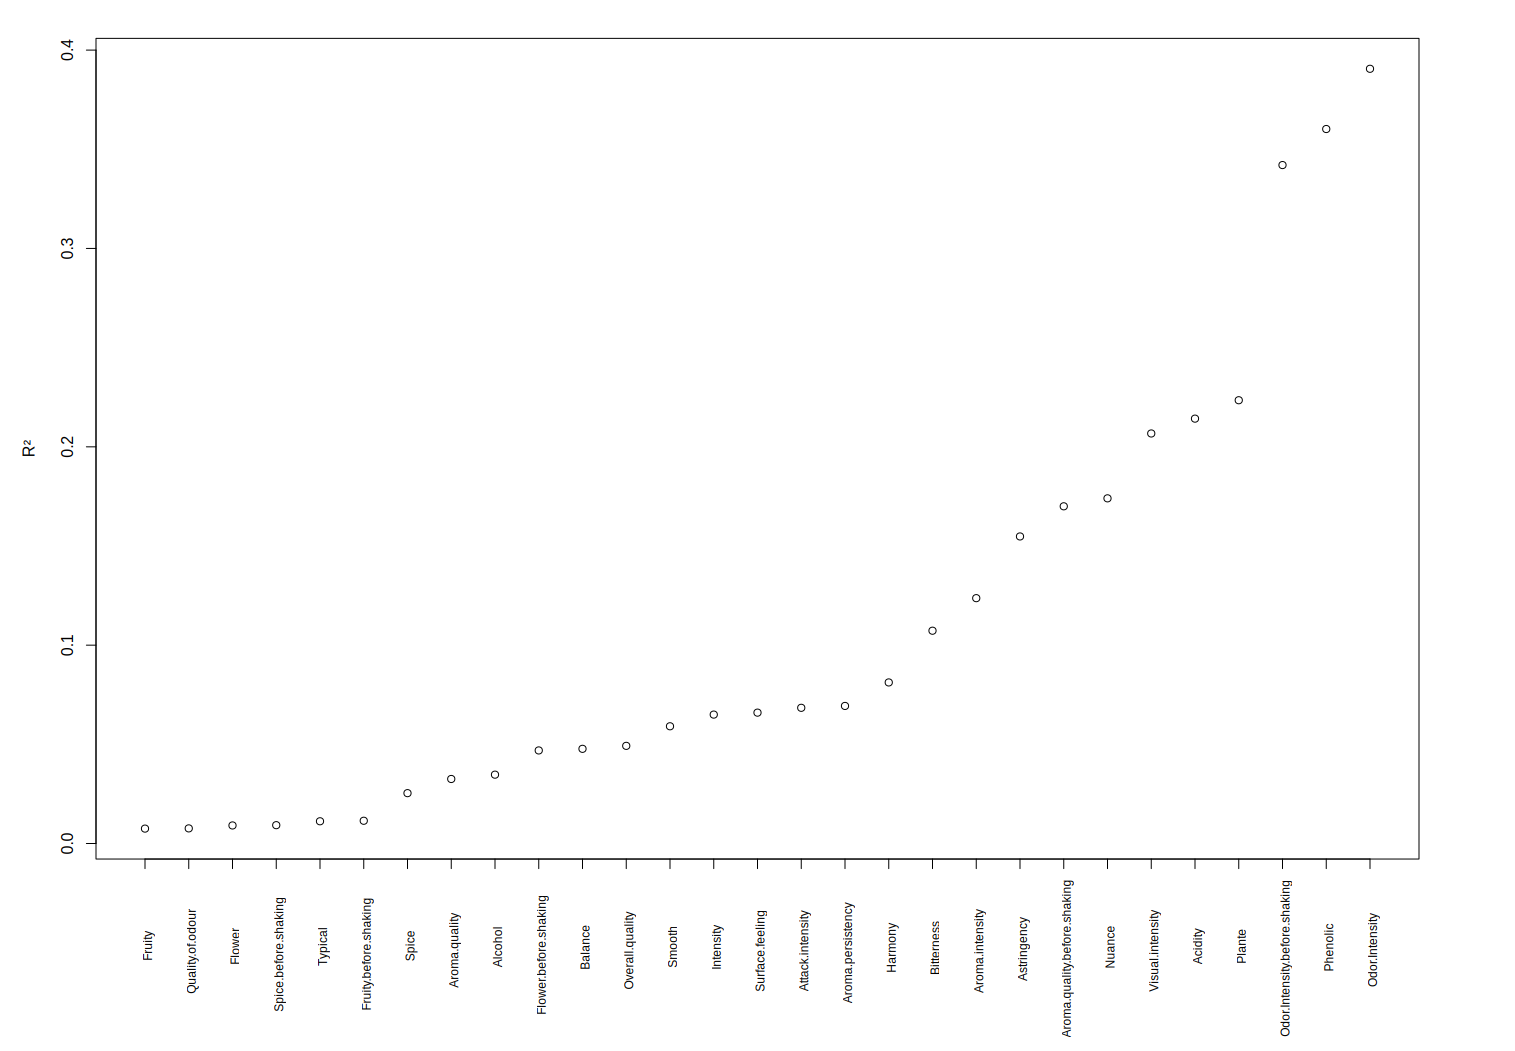
\includegraphics[width=0.85\linewidth]{Rplot04}
\end{center}

\textbf{Variables les plus liées à l'appellation :} 
	\begin{itemize}
	\item[$\bullet$] Odor.Intensity : 0.391
	\item[$\bullet$] Phenolic : 0.360
	\item[$\bullet$] Odor.Intensity.before.shaking 0.342
	\end{itemize}
	
\textbf{Variables les moins liées à l'appellation :}

\begin{itemize}
\item[$\bullet$] Fruity : 0.007
\item[$\bullet$] Quality.of.odour : 0.008 
\end{itemize}




Montrons que le $R^2_{\text{appellation}}$ est égal à la moyenne arithmétique des $R^2$ des variables que l'on notera~$M$. 
\begin{align*}
M=& \frac{1}{29} \sum_{j=1}^{29} \frac{\text{Variance externe de la variable } j }{\text{Variance totale de la variable } j} \\ 
 =& \frac{1}{29} \sum_{j=1}^{29} \frac{\sum_{k=1}^3 W^k\left(\overline{z^j}^k\right)^2}{1} \\
  =&\frac{1}{29} \sum_{k=1}^3  W^k \sum_{j=1}^{29} \left(\overline{z^j}^k\right)^2 \\
   =& \frac{1}{29} \sum_{k=1}^3 W^k \norme{\overline{z}^k}^2\\
 =& R^2_{\text{appellation}}
\end{align*}

Informatiquement, nous avons en premier lieu calculé la variance interne de chaque appellation, ce qui nous a permis d'obtenir ensuite un vecteur ligne à 29 colonnes : rvar. Puis en sommant ces valeurs et en divisant par le nombre de valeurs, ici 29, nous avons bien retrouvé la valeur du $R^2_{\text{appellation}}$ de la question \textbf{2.} :

\begin{center}
\begin{tabular}{|>{\centering\arraybackslash}p{2cm}|>{\centering\arraybackslash}p{2cm}|}
\hline 
$R$ & moy\_rvar \\ 
\hline 
0,109 & 0,109 \\ 
\hline 
\end{tabular} 
\end{center}
\end{enumerate}

\section{Partie 2}

Dans cette partie on notera $(x^j)$ les vecteurs colonnes de $X$. 

\begin{enumerate}
\item 
	\begin{enumerate}
	\item On considère le vecteur $\mathds{1}_n=\begin{pmatrix}
	1 \\ 
	\vdots \\ 
	 \\ 
	1
	\end{pmatrix} \in\mathbb{R}^{n}$.\\
	 On rappelle que $\mathds{1}_n\in \text{Vect}\left(y^1;...;y^p\right)=\langle Y \rangle$ car $\forall i\in\{1;...;n\},\, \sum_{j=1}^p \mathds{1}_{Y_i=j}=1$ donc $\mathds{1}_n\in \langle Y \rangle$.
Soit $j\in\{1;...;p\}$ :
	\begin{align*}
	\Pi_{\langle Y \rangle} x^j =& \Pi_{\langle\mathds{1}_n\rangle}x^j +\Pi_{\langle \mathds{1}_n^{\perp} \cap Y \rangle} x^j  \text{ car } \langle Y \rangle = \langle \mathds{1}_n \rangle \overset{\perp}{\oplus}\langle \mathds{1}_n^{\perp} \cap Y \rangle \\
	  =& 0 + \Pi_{\langle Y^c \rangle} x^j \\
	  =& \Pi_{\langle Y^c \rangle} x^j
	\end{align*}
 $\Pi_{\langle\mathds{1}_n\rangle}x^j=0$ car $x^j$ étant centré réduit, il appartient à $\mathds{1}_n^{\perp}$.

\begin{align*}
\norme{\Pi_Y x^j}^2_{W} =& \norme{\sum_{j=1}^n \overline{x}^j y_j}^2 \\
=& \sum_{j=1}^n \norme{\overline{x}^j y_j}^2 \text{ par orthogonalité des $y_j$} \\
					   =& \sum_{j=1}^n \sum_{i/Y_i=j} w_i (\overline{x}^{Y_i})^2 \\ 
					   =& \sum_{j=1}^n W^j (\overline{x}^j)^2 
\end{align*}
 
 
 
	
	$\norme{\Pi_Yx^j}^2_{W}$ représente la variance de la variable $x^j$ par rapport à l'appellation.
	
	\item $\Pi_Y=Y\left(Y'WY\right)^{-1}Y'W$  et $\Pi_{x^j}=x^{j}\left({x^{j}}'Wx^{j}\right)^{-1}{x^{j}}'W$ sont des matrices carrées de taille $21$.\\

\begin{align*}
\tr(\Pi_x^j \Pi_Y) =& \tr(\left(x^j\left( {x^j}' W x^j\right)^{-1} {x^j}' W \Pi_Y \right) \\
				   =& \frac{1}{\norme{x^j}_{W}^2} \tr\left(x^j {x^j}' W \Pi_Y\right) \\
				   =& \frac{1}{\norme{x^j}_{W}^2} \tr\left( {x^j}' W \Pi_Y x^j\right) \\
				   =& \frac{1}{\norme{x^j}_{W}^2}  {x^j}' W \Pi_Y x^j \text{ car } {x^j}' W \Pi_Y x^j \in \mathds{R} \\
				   =& \frac{1}{\norme{x^j}_{W}^2}  {x^j}' W \Pi_Y \Pi_Y x^j \\
				   =& \frac{1}{\norme{x^j}_{W}^2}  {x^j}' {\Pi_Y}' W  \Pi_Y x^j \\ 
				   =& \frac{\norme{\Pi x^j}_{W}^2}{\norme{x^j}_{W}^2} \\
				   =& R^2(x^j | Y)	     
\end{align*}	
	
	Cette dernière quantité représente le $R^2(x^j | Y)$ de la $j$-ème variable dans la partition des données en appellation. C'est $j$-ème valeur de notre variable informatique rvar.
	
	Voici un extrait de $\text{tr}(\Pi_x^j \Pi_Y)$ :	
	
	\item \begin{align*}
	 \tr(R \Pi_Y)=&\sum_{j=1}^p  \tr(R \Pi_{y^j}) \text{ car } Y=\overset{\perp}{\oplus} y^j \\
	 =& \sum_{j=1}^p \tr(\Pi_{y^j} R ) \\
	 =& \sum_{j=1}^p \tr(y^j({y^j}'Wy^j)^{-1}{y^j}'WXMX'W)\\
	 =& \sum_{j=1}^p \frac{1}{\norme{y^j}_W^2} \tr(y^j {y^j}'WXMX'W) \\
	 =& \sum_{j=1}^p \frac{1}{\frac{n_{j}}{n}} \tr({y^j}'WXMX'Wy^j ) \text{ où } n_{j}= \#(i/y_{i}^j=1)\\
	 =& \sum_{j=1}^p \frac{n_{n}}{n_j}\norme{{y^j}'WX}_M^2 \\
	 =& \sum_{j=1}^p \frac{n}{n_j}\times \frac{1}{n^2} \norme{y^jX}_M^2\\
	 =& \sum_{j=1}^p \frac{1}{n n_{j}} \times \frac{1}{p} \times \norme{{y^j}'X}^2 \\
	 =& \frac{1}{p} \sum_{j=1}^p \frac{n_{j}}{n} \norme{{y^j}' X / n_j}^2\\
	 =& \frac{1}{p} \sum_{j=1}^p W^j (\overline{x}^j)^2
	\end{align*}
	On retrouve donc ici la moyenne arithmétique des $R^2$ des variables ce qui correspond, d'après la partie 1, au $R^2_{\text{appellation}}$.
	
	Informatiquement, on obtient de nouveau $0,109$.
	
	\item Conclusion, à travers ces calculs matriciels, nous avons établi une correspondance entre les valeurs de la première partie et celles de la seconde, comme l'illustre le tableau suivant : 
	
	% \usepackage{array} is required
	\begin{center}
	\begin{tabular}{|m{3cm}|>{\centering\arraybackslash}m{5cm}|>{\centering\arraybackslash}m{5cm}|}
	\hline 
	 & Partie 1 & Partie 2 \\ 
	\hline 
$\sigma_{x^j}^2$ inter-appellation	 & Variance inter-appellation de la $j$-ème variable. & $\norme{ \Pi_Y x^j}$ \\ 
	\hline 
	$R^2(x^j|Y)$ & $R^2$ de la $j$-ème variable par rapport à l'appellation  & $\text{tr}(\Pi_{x^j}\Pi_{Y})$ \\ 
	\hline 
	$R^2_{\text{appellation}}$ & $R^2_{\text{appellation}}$ & $\text{tr}(R\Pi_Y)$ \\ 
	\hline 
	\end{tabular} 
	\end{center}
	\end{enumerate}
	

\item De la même façon, $\text{tr}(\Pi_{x^j}\Pi_{Z})$ est $R^2$ de la $j$-ème variable conditionné par le type de sol. $\text{tr}(R\Pi_{Z})$ est le $R^2$ de la partition des vins selon le type de sol.

Informatiquement, on trouve : $R^2_{\text{sol}}=0.365$.
\end{enumerate}

\newpage

\appendix 

\section{Code R}

\begin{lstlisting}[language=R]
library(xtable)
wine=read.csv('~/ADM/ADM-TP1/wine.csv')
xtable(wine[1:4,1:5], type = "latex", file = "wine.tex",digits = 3,
       caption = "Extrait du tableau")

#Mean and standard-deviation of the 29 quantitative variable in wine;
M = unname(colMeans(wine[4:32]))
V = unname(sapply(wine[4:32],sd))*sqrt(20/21) #variance corrigee ?? facteur (21/20) ?
print(V)
print(M)

#Centering and reducing
CR=wine
for (i in 1:29)
{
  CR[,3+i] <- (wine[,3+i]-M[i])/(V[i])
}
#Check if variables ar indeed recuded and centered
Barycentre=colMeans(CR[4:32])
Variance=diag(var(CR[4:32])*20/21)
print(Variance)
#inertia
Inertie=sum(Variance)
print(Inertie)

"Q2"
chinon=CR[CR$Label == 'Chinon',]
saumur=CR[CR$Label == 'Saumur',]
bourgueuil=CR[CR$Label == 'Bourgueuil',]

#poids
pchi=nrow(chinon)/nrow(CR)
psau=nrow(saumur)/nrow(CR)
pbou=nrow(bourgueuil)/nrow(CR)

#barycentre des classes 
mchi= (colMeans(chinon[4:32]))
msau= (colMeans(saumur[4:32]))
mbou= (colMeans(bourgueuil[4:32]))

#carree des normes euclidiennes des barycentres
nchi=sum(mchi^2)
nsau=sum(msau^2)
nbou=sum(mbou^2)

#Inertie externe
Inex=pchi*nchi+psau*nsau+pbou*nbou
Inex
#R2 pour le partitionement en appellation
R=Inex/Inertie
print(100*R)

#R2 par variable
rvar=pchi*mchi^2+psau*msau^2+pbou*mbou^2  #via normes euclidiennes
print(rvar)
trirvar=rvar[order(unlist(rvar))]
trirvar
plot(trirvar,xaxt='n')
axis(1,at=1:29,labels=FALSE,srt=90)
text(0.5:28.5,rep(-0.05,2),labels=names(trirvar),srt = 45,xpd=NA,adj=c(1,1))
sum(rvar*1/29) 

#PART2

#Q1
#def
w=1/nrow(wine) * diag(1,nrow(wine))
m=1/ncol(wine[4:32]) * diag(1,ncol(wine[4:32]))
X=as.matrix(CR[4:32])
Y=cbind(ifelse(CR$Label == 'Bourgueuil',1,0),ifelse(CR$Label == 
'Chinon',1,0),ifelse(CR$Label == 'Saumur',1,0))
Z=cbind(ifelse(CR$Soil == 'Env1',1,0),ifelse(CR$Soil == 'Env2',
1,0),ifelse(CR$Soil == 'Reference',1,0),ifelse(CR$Soil == 'Env4',1,0))

#piYw
Py= Y %*% solve(t(Y) %*% w %*% Y) %*% t(Y) %*% w
print(Py)

#piXjw
rm(j)
Px=list()
for (j in 1:29) {
  Px[[j]] = X[,j] %*% solve(t(X[,j]) %*% w %*% X[,j]) %*% t(X[,j]) %*% w
}
#tr
for (i in 1:29)
{
  T[i]=sum(diag(Px[[i]]%*%Py))
}

print(T)
print(unname(rvar))
# Coincide bien avec rvar de la premiere partie

#QC
Rma=X %*% m %*% t(X) %*% w
sum(diag(Rma %*% Py))

#Q2
Pz= Z %*% solve(t(Z) %*% w %*% Z) %*% t(Z) %*% w
sum(diag(Rma %*% Pz))
\end{lstlisting}

\end{document}
